\chapter{概率}

\index{概率}

\key{概率}是一个介于$0$和$1$之间的实数，
表示一个事件发生的可能性。
如果一个事件一定会发生，
其概率为1；
如果一个事件不可能发生，
其概率为0。
事件的概率记为$P(\cdots)$，
其中三个点描述该事件。

例如，掷骰子时，
结果是一个介于$1$和$6$之间的整数，
每个结果的概率为$1/6$。
例如，我们可以计算以下概率：

\begin{itemize}[noitemsep]
\item $P(\textrm{''结果为4''})=1/6$
\item $P(\textrm{''结果不为6''})=5/6$
\item $P(\textrm{''结果为偶数''})=1/2$
\end{itemize}

\section{计算}

要计算一个事件的概率，
我们可以使用组合数学
或模拟生成该事件的过程。
例如，让我们计算
从洗好的牌堆中抽出三张点数相同的牌
的概率
（例如，$\spadesuit 8$、$\clubsuit 8$和$\diamondsuit 8$）。

\subsubsection*{方法1}

我们可以使用以下公式计算概率

\[\frac{\textrm{期望结果的数量}}{\textrm{总结果数}}.\]

在这个问题中，期望结果是
每张牌的点数相同的情况。
这样的结果有$13 {4 \choose 3}$种，
因为牌的点数有$13$种可能，
从4种花色中选择3种
有${4 \choose 3}$种方式。

总共有${52 \choose 3}$种结果，
因为我们要从52张牌中选3张。
因此，该事件的概率为

\[\frac{13 {4 \choose 3}}{{52 \choose 3}} = \frac{1}{425}.\]

\subsubsection*{方法2}

另一种计算概率的方法是
模拟生成该事件的过程。
在这个例子中，我们抽三张牌，因此该过程
由三步组成。
我们要求每一步都成功。

抽第一张牌显然成功，
因为没有限制。
第二步成功的概率为$3/51$，
因为还剩51张牌，其中3张
与第一张牌点数相同。
类似地，第三步成功的概率为$2/50$。

整个过程成功的概率为

\[1 \cdot \frac{3}{51} \cdot \frac{2}{50} = \frac{1}{425}.\]

\section{事件}

概率论中的一个事件可以表示为一个集合
\[A \subset X,\]
其中$X$包含所有可能的结果，
而$A$是结果的一个子集。
例如，掷骰子时，结果为
\[X = \{1,2,3,4,5,6\}.\]
现在，例如事件''结果为偶数''
对应的集合为
\[A = \{2,4,6\}.\]

每个结果$x$被赋予一个概率$p(x)$。
那么，事件$A$的概率$P(A)$
可以用以下公式计算为
结果概率之和
\[P(A) = \sum_{x \in A} p(x).\]
例如，掷骰子时，
每个结果$x$的$p(x)=1/6$，
因此事件''结果为偶数''
的概率为
\[p(2)+p(4)+p(6)=1/2.\]

$X$中所有结果的总概率必须
为1，即$P(X)=1$。

由于概率论中的事件是集合，
我们可以使用标准的集合运算来操作它们：

\begin{itemize}
\item \key{补集}$\bar A$表示
''$A$不发生''。
例如，掷骰子时，
$A=\{2,4,6\}$的补集为
$\bar A = \{1,3,5\}$。
\item \key{并集}$A \cup B$表示
''$A$或$B$发生''。
例如，$A=\{2,5\}$
和$B=\{4,5,6\}$的并集为
$A \cup B = \{2,4,5,6\}$。
\item \key{交集}$A \cap B$表示
''$A$和$B$同时发生''。
例如，$A=\{2,5\}$和$B=\{4,5,6\}$
的交集为
$A \cap B = \{5\}$。
\end{itemize}

\subsubsection{补集}

补集$\bar A$的概率
用以下公式计算
\[P(\bar A)=1-P(A).\]

有时，我们可以通过求解相反的问题
利用补集来轻松求解问题。
例如，掷骰子十次至少出现一次6的概率为
\[1-(5/6)^{10}.\]

这里$5/6$是单次掷骰
结果不为6的概率，
而$(5/6)^{10}$是十次掷骰
中没有一次是6的概率。
其补集即为问题的答案。

\subsubsection{并集}

并集$A \cup B$的概率
用以下公式计算
\[P(A \cup B)=P(A)+P(B)-P(A \cap B).\]
例如，掷骰子时，
事件
\[A=\textrm{''结果为偶数''}\]
和
\[B=\textrm{''结果小于4''}\]
的并集为
\[A \cup B=\textrm{''结果为偶数或小于4''},\]
其概率为
\[P(A \cup B) = P(A)+P(B)-P(A \cap B)=1/2+1/2-1/6=5/6.\]

如果事件$A$和$B$是\key{互斥}的，即
$A \cap B$为空集，
那么事件$A \cup B$的概率就是

\[P(A \cup B)=P(A)+P(B).\]

\subsubsection{条件概率}

\index{条件概率}

\key{条件概率}
\[P(A | B) = \frac{P(A \cap B)}{P(B)}\]
是在假设$B$发生时
$A$的概率。
因此，在计算$A$的概率时，
我们只考虑也属于$B$的结果。

使用前面的集合，
\[P(A | B)= 1/3,\]
因为$B$的结果为
$\{1,2,3\}$，其中一个是偶数。
这是当我们知道结果在$1 \ldots 3$之间时，
结果为偶数的概率。

\subsubsection{交集}

\index{独立性}

利用条件概率，
交集$A \cap B$的概率
可以用以下公式计算
\[P(A \cap B)=P(A)P(B|A).\]
如果事件$A$和$B$是\key{独立}的，即
\[P(A|B)=P(A) \hspace{10pt}\textrm{且}\hspace{10pt} P(B|A)=P(B),\]
这意味着$B$的发生不改变
$A$的概率，反之亦然。
在这种情况下，交集的概率为
\[P(A \cap B)=P(A)P(B).\]
例如，从牌堆中抽一张牌时，事件
\[A = \textrm{''花色为梅花''}\]
和
\[B = \textrm{''点数为4''}\]
是独立的。因此事件
\[A \cap B = \textrm{''这张牌是梅花4''}\]
发生的概率为
\[P(A \cap B)=P(A)P(B)=1/4 \cdot 1/13 = 1/52.\]

\section{随机变量}

\index{随机变量}

\key{随机变量}是一个由随机过程
生成的值。
例如，掷两颗骰子时，
一个可能的随机变量是
\[X=\textrm{''结果之和''}.\]
例如，如果结果是$[4,6]$
（即我们第一次掷出4，第二次掷出6），
那么$X$的值为10。

我们用$P(X=x)$表示
随机变量$X$的值为$x$的概率。
例如，掷两颗骰子时，
$P(X=10)=3/36$，
因为总结果数为36，
而得到和为10的方式有三种：
$[4,6]$、$[5,5]$和$[6,4]$。

\subsubsection{期望值}

\index{期望值}

\key{期望值}$E[X]$表示
随机变量$X$的平均值。
期望值可以计算为以下求和
\[\sum_x P(X=x)x,\]
其中$x$遍历$X$的所有可能值。

例如，掷骰子时，
期望结果为
\[1/6 \cdot 1 + 1/6 \cdot 2 + 1/6 \cdot 3 + 1/6 \cdot 4 + 1/6 \cdot 5 + 1/6 \cdot 6 = 7/2.\]

期望值的一个有用性质是\key{线性性}。
这意味着和
$E[X_1+X_2+\cdots+X_n]$
始终等于和
$E[X_1]+E[X_2]+\cdots+E[X_n]$。
即使随机变量相互依赖，
该公式也成立。

例如，掷两颗骰子时，
期望和为
\[E[X_1+X_2]=E[X_1]+E[X_2]=7/2+7/2=7.\]

现在考虑一个问题：
$n$个球随机放入$n$个盒子中，
我们的任务是计算空盒子
的期望数量。
每个球放入任何
一个盒子的概率相等。
例如，如果$n=2$，可能的情况
如下：
\begin{center}
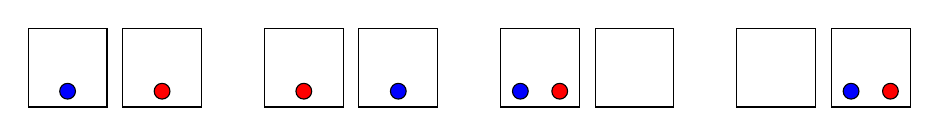
\begin{tikzpicture}
\draw (0,0) rectangle (1,1);
\draw (1.2,0) rectangle (2.2,1);
\draw (3,0) rectangle (4,1);
\draw (4.2,0) rectangle (5.2,1);
\draw (6,0) rectangle (7,1);
\draw (7.2,0) rectangle (8.2,1);
\draw (9,0) rectangle (10,1);
\draw (10.2,0) rectangle (11.2,1);

\draw[fill=blue] (0.5,0.2) circle (0.1);
\draw[fill=red] (1.7,0.2) circle (0.1);
\draw[fill=red] (3.5,0.2) circle (0.1);
\draw[fill=blue] (4.7,0.2) circle (0.1);
\draw[fill=blue] (6.25,0.2) circle (0.1);
\draw[fill=red] (6.75,0.2) circle (0.1);
\draw[fill=blue] (10.45,0.2) circle (0.1);
\draw[fill=red] (10.95,0.2) circle (0.1);
\end{tikzpicture}
\end{center}
在这种情况下，空盒子的期望数量为
\[\frac{0+0+1+1}{4} = \frac{1}{2}.\]
在一般情形下，单个盒子为空的概率为
\[\Big(\frac{n-1}{n}\Big)^n,\]
因为没有球被放入其中。
因此，利用线性性，空盒子的期望数量为
\[n \cdot \Big(\frac{n-1}{n}\Big)^n.\]

\subsubsection{分布}

\index{分布}

随机变量$X$的\key{分布}
展示了$X$可能取的
每个值的概率。
分布由值$P(X=x)$组成。
例如，掷两颗骰子时，
它们的和的分布为：
\begin{center}
\small {
\begin{tabular}{r|rrrrrrrrrrrrr}
$x$ & 2 & 3 & 4 & 5 & 6 & 7 & 8 & 9 & 10 & 11 & 12 \\
$P(X=x)$ & $1/36$ & $2/36$ & $3/36$ & $4/36$ & $5/36$ & $6/36$ & $5/36$ & $4/36$ & $3/36$ & $2/36$ & $1/36$ \\
\end{tabular}
}
\end{center}

\index{均匀分布}
在\key{均匀分布}中，
随机变量$X$有$n$个可能的
值$a,a+1,\ldots,b$，每个值的概率为$1/n$。
例如，掷骰子时，
$a=1$，$b=6$，每个值$x$的$P(X=x)=1/6$。

均匀分布中$X$的期望值为
\[E[X] = \frac{a+b}{2}.\]

\index{二项分布}
在\key{二项分布}中，进行$n$次尝试，
每次尝试成功的概率
为$p$。
随机变量$X$计算成功尝试的次数，
值$x$的概率为
\[P(X=x)=p^x (1-p)^{n-x} {n \choose x},\]
其中$p^x$和$(1-p)^{n-x}$对应于
成功和失败的尝试，
而${n \choose x}$是我们
可以选择尝试顺序的方式数。

例如，掷骰子十次时，
恰好掷出三次6的概率为$(1/6)^3 (5/6)^7 {10 \choose 3}$。

二项分布中$X$的期望值为
\[E[X] = pn.\]

\index{几何分布}
在\key{几何分布}中，
一次尝试成功的概率为$p$，
我们持续尝试直到第一次成功。
随机变量$X$计算所需的尝试次数，
值$x$的概率为
\[P(X=x)=(1-p)^{x-1} p,\]
其中$(1-p)^{x-1}$对应于失败的尝试，
$p$对应于第一次成功的尝试。

例如，如果我们掷骰子直到掷出6，
掷骰次数恰好为4的概率为$(5/6)^3 1/6$。

几何分布中$X$的期望值为
\[E[X]=\frac{1}{p}.\]

\section{马尔可夫链}

\index{马尔可夫链}

\key{马尔可夫链}
% \footnote{A. A. Markov (1856--1922)
% 是一位俄罗斯数学家。}
是一个随机过程，
由状态和状态之间的转移组成。
对于每个状态，我们知道
转移到其他状态的概率。
马尔可夫链可以表示为一个图，
其节点是状态，边是转移。

作为一个例子，考虑一个问题：
我们在一栋$n$层建筑的第1层。
每一步，我们随机走上一层
或下一层，但从第1层我们总是
走上一层，从第$n$层
我们总是走下一层。
经过$k$步后，在第$m$层的概率是多少？

在这个问题中，建筑的每层
对应于马尔可夫链中的一个状态。
例如，如果$n=5$，图如下：

\begin{center}
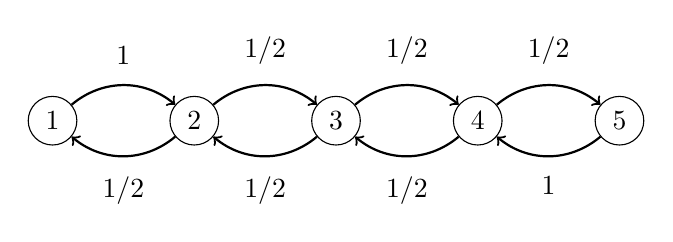
\begin{tikzpicture}[scale=0.9]
\node[draw, circle] (1) at (0,0) {$1$};
\node[draw, circle] (2) at (2,0) {$2$};
\node[draw, circle] (3) at (4,0) {$3$};
\node[draw, circle] (4) at (6,0) {$4$};
\node[draw, circle] (5) at (8,0) {$5$};

\path[draw,thick,->] (1) edge [bend left=40] node[font=\small,label=$1$] {} (2);
\path[draw,thick,->] (2) edge [bend left=40] node[font=\small,label=$1/2$] {} (3);
\path[draw,thick,->] (3) edge [bend left=40] node[font=\small,label=$1/2$] {} (4);
\path[draw,thick,->] (4) edge [bend left=40] node[font=\small,label=$1/2$] {} (5);

\path[draw,thick,->] (5) edge [bend left=40] node[font=\small,label=below:$1$] {} (4);
\path[draw,thick,->] (4) edge [bend left=40] node[font=\small,label=below:$1/2$] {} (3);
\path[draw,thick,->] (3) edge [bend left=40] node[font=\small,label=below:$1/2$] {} (2);
\path[draw,thick,->] (2) edge [bend left=40] node[font=\small,label=below:$1/2$] {} (1);

%\path[draw,thick,->] (1) edge [bend left=40] node[font=\small,label=below:$1$] {} (2);
\end{tikzpicture}
\end{center}

马尔可夫链的概率分布
是一个向量
$[p_1,p_2,\ldots,p_n]$，其中$p_k$是
当前状态为$k$的概率。
公式$p_1+p_2+\cdots+p_n=1$始终成立。

在上述场景中，初始分布为
$[1,0,0,0,0]$，因为我们始终从第1层开始。
下一个分布为$[0,1,0,0,0]$，
因为我们只能从第1层移动到第2层。
之后，我们可以走上一层
或下一层，因此下一个分布为
$[1/2,0,1/2,0,0]$，以此类推。

模拟马尔可夫链中行走的一种高效方法
是使用动态规划。
其思想是维护概率分布，
并在每一步遍历所有
可能的移动方式。
使用这种方法，我们可以在
$O(n^2 m)$时间内模拟$m$步的行走。

马尔可夫链的转移也可以
表示为一个矩阵，用以更新
概率分布。
在上述场景中，矩阵为

\[ 
 \begin{bmatrix}
  0 & 1/2 & 0 & 0 & 0 \\
  1 & 0 & 1/2 & 0 & 0 \\
  0 & 1/2 & 0 & 1/2 & 0 \\
  0 & 0 & 1/2 & 0 & 1 \\
  0 & 0 & 0 & 1/2 & 0 \\
 \end{bmatrix}.
\]

当我们用这个矩阵乘以概率分布时，
我们得到移动一步后的新分布。
例如，我们可以从分布
$[1,0,0,0,0]$转移到分布
$[0,1,0,0,0]$，如下所示：

\[ 
 \begin{bmatrix}
  0 & 1/2 & 0 & 0 & 0 \\
  1 & 0 & 1/2 & 0 & 0 \\
  0 & 1/2 & 0 & 1/2 & 0 \\
  0 & 0 & 1/2 & 0 & 1 \\
  0 & 0 & 0 & 1/2 & 0 \\
 \end{bmatrix}
 \begin{bmatrix}
  1 \\
  0 \\
  0 \\
  0 \\
  0 \\
 \end{bmatrix}
=
 \begin{bmatrix}
  0 \\
  1 \\
  0 \\
  0 \\
  0 \\
 \end{bmatrix}.
\]

通过高效地计算矩阵幂，
我们可以在$O(n^3 \log m)$时间内
计算$m$步后的分布。

\section{随机化算法}

\index{随机化算法}

有时我们可以利用随机性来解决问题，
即使问题与概率无关。
\key{随机化算法}是一种
基于随机性的算法。

\index{蒙特卡洛算法}

\key{蒙特卡洛算法}是一种随机化算法，
可能有时会给出错误的答案。
要使这种算法有用，
给出错误答案的概率应该很小。

\index{拉斯维加斯算法}

\key{拉斯维加斯算法}是一种随机化算法，
始终给出正确答案，
但其运行时间随机变化。
目标是以高概率设计一个
高效的算法。

接下来我们将介绍三个可以使用随机性
解决的示例问题。

\subsubsection{顺序统计量}

\index{顺序统计量}

数组的第$k$个\key{顺序统计量}
是将数组按递增顺序排序后
位于位置$k$的元素。
我们可以通过先对数组排序
在$O(n \log n)$时间内计算任意顺序统计量，
但真的需要为了找一个元素
而对整个数组排序吗？

事实上，我们可以使用随机化算法
在不排序的情况下找到顺序统计量。
该算法称为\key{快速选择}
\footnote{1961年，
C. A. R. Hoare发表了两个平均效率
很高的算法：\index{快速排序} \index{快速选择}
\key{快速排序}\cite{hoa61a}用于数组排序，
\key{快速选择}\cite{hoa61b}用于寻找顺序统计量。}，
是一个拉斯维加斯算法：
其运行时间通常为$O(n)$，
但最坏情况下为$O(n^2)$。

该算法选择数组中的一个随机元素$x$，
将小于$x$的元素移到数组的左半部分，
其他所有元素移到右半部分。
当有$n$个元素时，这需要$O(n)$时间。
假设左半部分包含$a$个元素，
右半部分包含$b$个元素。
如果$a=k$，元素$x$就是第$k$个顺序统计量。
否则，如果$a>k$，我们递归地在左半部分找第$k$个顺序统计量，
如果$a<k$，我们递归地在右半部分找第$r$个顺序统计量，
其中$r=k-a$。
搜索以类似的方式继续，直到找到
该元素。

当每个元素$x$随机选取时，
数组大小在每一步大约减半，
因此找第$k$个顺序统计量的时间复杂度约为
\[n+n/2+n/4+n/8+\cdots < 2n = O(n).\]

该算法的最坏情况仍然需要$O(n^2)$时间，
因为有可能$x$总是被选择为
数组中最小或最大的元素之一，
需要$O(n)$步。
然而，这种情况的概率如此之小，
以至于在实际中从未发生。

\subsubsection{验证矩阵乘法}

\index{矩阵乘法}

我们的下一个问题是\emph{验证}
当$A$、$B$和$C$是$n \times n$矩阵时
$AB=C$是否成立。
当然，我们可以通过重新计算乘积$AB$
（使用基本算法需$O(n^3)$时间）
来解决问题，
但人们可能希望验证答案
比从头计算更容易。

事实上，我们可以使用蒙特卡洛算法
\footnote{R. M. Freivalds于1977年发表了
该算法\cite{fre77}，有时
称为\index{Freivalds算法} \key{Freivalds算法}。}
来解决问题，其时间复杂度仅为$O(n^2)$。
思想很简单：我们选择一个由
$n$个元素组成的随机向量$X$，并计算矩阵
$ABX$和$CX$。如果$ABX=CX$，我们报告$AB=C$，
否则报告$AB \neq C$。

该算法的时间复杂度为
$O(n^2)$，因为我们可以在$O(n^2)$时间内
计算矩阵$ABX$和$CX$。
我们可以利用$A(BX)$的表示高效地
计算矩阵$ABX$，因此只需要两次
$n \times n$和$n \times 1$大小矩阵的乘法。

该算法的缺点是
当它报告$AB=C$时，算法有很小的
几率犯错。
例如，
\[
 \begin{bmatrix}
  6 & 8 \\
  1 & 3 \\
 \end{bmatrix}
\neq
 \begin{bmatrix}
  8 & 7 \\
  3 & 2 \\
 \end{bmatrix},
\]
但
\[
 \begin{bmatrix}
  6 & 8 \\
  1 & 3 \\
 \end{bmatrix}
 \begin{bmatrix}
  3 \\
  6 \\
 \end{bmatrix}
=
 \begin{bmatrix}
  8 & 7 \\
  3 & 2 \\
 \end{bmatrix}
 \begin{bmatrix}
  3 \\
  6 \\
 \end{bmatrix}.
\]
但在实践中，算法犯错
的概率很小，
并且我们可以通过使用多个随机向量$X$
验证结果来降低概率，
然后再报告$AB=C$。

\subsubsection{图着色}

\index{着色}

给定一个包含$n$个节点和$m$条边的图，
我们的任务是找到一种用两种颜色
为图的节点着色的方法，使得
至少$m/2$条边的两个端点
颜色不同。
例如，在图
\begin{center}
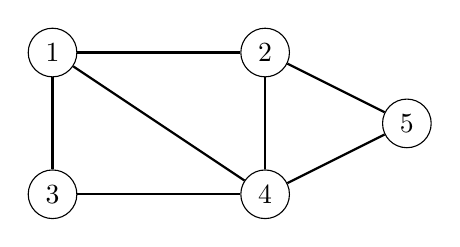
\begin{tikzpicture}[scale=0.9]
\node[draw, circle] (1) at (1,3) {$1$};
\node[draw, circle] (2) at (4,3) {$2$};
\node[draw, circle] (3) at (1,1) {$3$};
\node[draw, circle] (4) at (4,1) {$4$};
\node[draw, circle] (5) at (6,2) {$5$};

\path[draw,thick,-] (1) -- (2);
\path[draw,thick,-] (1) -- (3);
\path[draw,thick,-] (1) -- (4);
\path[draw,thick,-] (3) -- (4);
\path[draw,thick,-] (2) -- (4);
\path[draw,thick,-] (2) -- (5);
\path[draw,thick,-] (4) -- (5);
\end{tikzpicture}
\end{center}
中，一个有效的着色如下：
\begin{center}
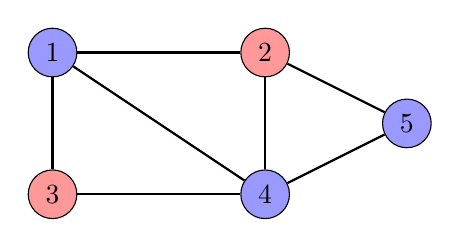
\begin{tikzpicture}[scale=0.9]
\node[draw, circle, fill=blue!40] (1) at (1,3) {$1$};
\node[draw, circle, fill=red!40] (2) at (4,3) {$2$};
\node[draw, circle, fill=red!40] (3) at (1,1) {$3$};
\node[draw, circle, fill=blue!40] (4) at (4,1) {$4$};
\node[draw, circle, fill=blue!40] (5) at (6,2) {$5$};

\path[draw,thick,-] (1) -- (2);
\path[draw,thick,-] (1) -- (3);
\path[draw,thick,-] (1) -- (4);
\path[draw,thick,-] (3) -- (4);
\path[draw,thick,-] (2) -- (4);
\path[draw,thick,-] (2) -- (5);
\path[draw,thick,-] (4) -- (5);
\end{tikzpicture}
\end{center}
上面的图包含7条边，其中5条边
的两个端点颜色不同，
因此该着色是有效的。

该问题可以使用拉斯维加斯算法解决，
该算法生成随机着色，直到找到
有效的着色。
在随机着色中，每个节点的颜色
独立选择，两种颜色的
概率均为$1/2$。

在随机着色中，单条边的两个端点
颜色不同的概率为$1/2$。
因此，端点颜色不同的边
的期望数量为$m/2$。
由于随机着色的期望是有效的，
在实践中我们会很快找到有效的着色。

